\documentclass[11pt]{article}
% Official ACL template (acl.sty in final mode, acl_natbib.bst). Citations are numeric through natbib's own
% package options; the template files are unmodified.
\PassOptionsToPackage{numbers,square,sort&compress}{natbib}
\usepackage[final]{acl}
\usepackage{times}
\usepackage{latexsym}
\usepackage[T1]{fontenc}
\usepackage[utf8]{inputenc}
\usepackage{microtype}
\usepackage{inconsolata}
\usepackage{graphicx}
\usepackage{booktabs}
\usepackage{amsmath}
\usepackage{amssymb}
\usepackage{array}

\newcommand{\dact}{\textsc{Dact}}

\title{Difference-Aware Contrastive Transformer for\\Physical Commonsense Question Answering}

\author{Group 73}

\begin{document}
\maketitle

\begin{abstract}
Can a neural model trained from scratch answer physical commonsense questions more accurately when the differences between the candidate answers are modelled explicitly? We study this question with the Difference-Aware Contrastive Transformer (\dact{}). \dact{} marks the tokens on which two near-identical candidate solutions differ, compares the candidates with cross-solution attention, pools each candidate around its differing tokens and adds a jointly trained lexical score. On PIQA we compare it with five baselines and nine ablations. \dact{} reaches the highest validation accuracy among the models trained from scratch (61.3\%), but on the evaluation split its accuracy is not significantly different from that of a TF-IDF baseline (61.9 vs.\ 61.2\%, McNemar $p{=}0.62$). Most of the model's attention falls on the differing tokens, and wrong predictions attend to them slightly more than correct ones, so locating a difference is not enough to judge its physical plausibility.
\end{abstract}

\section{Introduction}

\subsection{Background and Motivation}
Physical commonsense, knowing how everyday objects behave and what they can be used for, is needed by assistants that give practical instructions and by robots that must choose feasible actions. PIQA \cite{bisk2020piqa} tests this knowledge in a question answering format: each item pairs an everyday goal with two candidate solutions, exactly one of which achieves it. What makes the task hard is that the two candidates are usually near-duplicates. In our training split, the median share of solution tokens that differ between them is 15\%, so the answer hinges on a few substituted words whose plausibility can only be judged with world knowledge. This is why we chose an architecture that represents the differences between the candidates explicitly instead of scoring each one on its own.

\subsection{Objectives and Main Findings}
We ask whether a model trained from scratch, with no external data, can make use of the explicit differences between two candidate solutions. We set out to (i) design an attention-based architecture that represents these differences at the input, comparison and pooling stages; (ii) compare it with baselines ranging from a majority classifier to pretrained models; (iii) measure what each component contributes through controlled ablations; and (iv) check whether the attention concentrates on the differing tokens and how that relates to the errors. We find that \dact{} is the strongest model trained from scratch on validation but not significantly better than a lexical baseline on the evaluation split, that its difference-aware components help only in combination, and that its errors seem to come from missing world knowledge rather than from misplaced attention.

\subsection{Related Work}
\citet{bisk2020piqa} report 77.1\% accuracy for RoBERTa-large and 94.9\% for humans, and training on many question answering formats improves pretrained models further \cite{khashabi2020unifiedqa}. Our model builds on the Transformer encoder \cite{vaswani2017attention}. In multiple-choice reading comprehension, the Option Comparison Network \cite{ran2019option} and DCMN+ \cite{zhang2020dcmn} compare the candidate answers with each other rather than scoring them independently. In natural language inference, ESIM \cite{chen2017esim} and the decomposable attention model \cite{parikh2016decomposable} align two texts token by token and build comparison features from that alignment. Work on annotation artefacts shows that shallow lexical cues can solve many items without reasoning \cite{gururangan2018annotation,poliak2018hypothesis}, which is why we include both a lexical baseline and a lexical component in the model.

\section{Methodology}\label{sec:method}
\begin{figure*}[t]
\centering
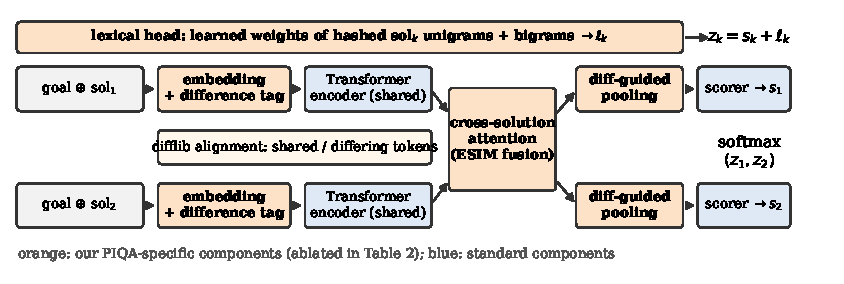
\includegraphics[width=0.97\textwidth]{figures/architecture.pdf}
\caption{Architecture of \dact{}. The two candidates share all weights, so swapping two already-encoded candidates swaps their scores. The \texttt{difflib} alignment that produces the tags does depend on the order of the options (Section~\ref{sec:limits}).}
\label{fig:arch}
\end{figure*}

\dact{} is a Transformer-based model trained from scratch on the PIQA training data alone (Figure~\ref{fig:arch}). The Transformer encoder, additive attention, byte-pair encoding and the ESIM comparison features come from prior work. Our contribution is to adapt and combine them for PIQA: difference-tag embeddings, a cross-solution comparison of the two competing solutions, difference-guided pooling, and a lexical scoring component trained jointly with the neural model.

\subsection{Task Formulation}
Each item has a goal $g$ and two candidate solutions $s_1$ and $s_2$. The model computes a score $z_k$ for each candidate $k \in \{1,2\}$ and predicts $\hat{y} = \arg\max_k z_k$.

\subsection{Input Representation and Difference Tags}
Each candidate is encoded as $x^{(k)} = [\textsc{cls}]\,g\,[\textsc{sep}]\,s_k\,[\textsc{sep}]$, using a byte-pair-encoding (BPE) vocabulary \cite{sennrich2016bpe} learned on the training split. We align the token sequences of $s_1$ and $s_2$ with Python's \texttt{difflib} and tag every solution token as \textit{shared} or \textit{different}; goal and special tokens get the tag \textit{other}. The input embedding at position $i$ is
\begin{equation}
e_i = E_{tok}[x_i] + E_{pos}[i] + E_{seg}[\sigma_i] + E_{tag}[t_i],
\end{equation}
followed by layer normalisation and dropout. Here $E_{tok}$, $E_{pos}$, $E_{seg}$ and $E_{tag}$ are learned token, position, segment and tag embeddings, $t_i$ is the tag at position $i$, and $\sigma_i$ indicates whether the position belongs to the goal or to the solution. The tag embedding tells the encoder from the first layer onwards where the candidates disagree. The tags assume that the candidates share most of their wording: for paraphrased candidates nearly every token is tagged as different, synonyms count as differences, and the alignment depends on the order of the options.

\subsection{Shared Transformer Encoder}
A pre-LayerNorm Transformer encoder \cite{vaswani2017attention,xiong2020layer} maps each candidate sequence to hidden states $H^{(k)} \in \mathbb{R}^{L \times d}$. Since both candidates go through the same encoder, any difference between their representations comes from the inputs, not from separate parameters.

\subsection{Cross-Solution Attention}
Plausibility in PIQA is relative: a solution is right because it is better than its rival. Each token of candidate $k$ therefore attends to the solution tokens of the other candidate $\bar{k}$ and to its \textsc{cls} token, which serves as a target when a token has no counterpart:
\begin{equation}
c_i = \mathrm{MHA}\big(\bar{h}^{(k)}_i, \bar{H}^{(\bar{k})}, \bar{H}^{(\bar{k})}\big),\quad \bar{h} = \mathrm{LN}(h),
\end{equation}
where MHA is multi-head attention with the keys restricted to these positions. The hidden states are then updated with ESIM's comparison features \cite{chen2017esim}: $\tilde{h}_i = \mathrm{LN}\big(h_i + \mathrm{FFN}([\bar{h}_i; c_i; \bar{h}_i - c_i; \bar{h}_i \odot c_i])\big)$. ESIM uses these features for premise--hypothesis pairs; we use them for two competing answers, so that each candidate is represented by what it contains in contrast to its rival.

\subsection{Difference-Guided Attention Pooling}
Additive attention \cite{bahdanau2015neural}, extended with a learned bias for each tag, summarises the solution tokens:
\begin{equation}
\alpha_i \propto \exp\big(v^\top \tanh(W \tilde{h}_i) + b_{t_i}\big),\quad p = \textstyle\sum_i \alpha_i \tilde{h}_i,
\end{equation}
where $v$ and $W$ are learned, $b_{\textit{different}}$ starts at 1 and the other biases at 0. At the start of training, the bias steers the summary towards the substituted tokens; Section~\ref{sec:attention} checks whether the trained model still relies on it. A scoring MLP maps $[p; \tilde{h}_{\textsc{cls}}]$ to a neural score $s_k$.

\subsection{Lexical Scoring Component}
Following the wide-and-deep idea \cite{cheng2016wide}, a sparse linear component scores the words of each solution directly. Every BPE unigram and bigram of $s_k$ is hashed into one of $2^{18}$ buckets, each with a learned weight $w_j$ initialised to 0:
\begin{equation}
\ell_k = \textstyle\sum_{j \in \mathrm{ngrams}(s_k)} w_{h(j)},\qquad z_k = s_k + \ell_k,
\end{equation}
where $h$ is the hash function. The prediction depends only on $z_1 - z_2$, so n-grams that appear in both candidates cancel out, and the component learns, much like a TF-IDF classifier, which substituted words signal a plausible solution. It is trained jointly with the Transformer but has its own learning rate.

\subsection{Prediction and Training Objective}
The two scores compete in a softmax, $P(k) = \mathrm{softmax}(z_1, z_2)_k$, trained with cross-entropy and label smoothing of 0.1. This pairwise objective fits PIQA's forced-choice format, in which exactly one candidate is correct. Before training on this objective, the selected configuration runs a 10-epoch masked-language-model (MLM) warm-up \cite{devlin2019bert} on the text of the training split.


\section{Experimental Setup}

\subsection{Dataset and Data Split}
PIQA provides 16{,}113 labelled training items and 1{,}838 labelled development items; the labels of the official test set are not public. The unit's test files are byte-identical to the development items (same SHA-256), and we use them as our evaluation split. We held out a stratified 10\% of the training file (seed 42) for validation, which gives 14{,}501 / 1{,}612 / 1{,}838 items for training, validation and evaluation, all label-balanced (50.0 / 50.0 / 50.5\% label 1). A data audit found six duplicate rows within the training file and one evaluation item (index 1545) that occurs twice in the training split. We kept the split unchanged and report the overlap: re-scoring the saved evaluation predictions without that item changes accuracy by about 0.02 points (\dact{} 61.86\,$\to$\,61.84\%, TF-IDF 61.21\,$\to$\,61.19\%).

\subsection{Data Preprocessing}
Whitespace is collapsed, and the BPE tokeniser applies NFKC normalisation and lower-casing. Goals are truncated to 40 BPE tokens and solutions to 96. For longer solutions (1.6\% of the evaluation solutions), the 96-token window is centred on the differing span rather than keeping the prefix.

\subsection{Training Configuration}
The final model has $d{=}128$, two layers, four attention heads and a feed-forward width of 512, for 1.93\,M parameters in total, 262\,k of them in the lexical component. We train it with AdamW \cite{loshchilov2019decoupled} ($\beta_2{=}0.98$, weight decay 0.05, learning rate $3{\times}10^{-4}$ and $10^{-2}$ for the lexical component), a 6\% linear warm-up followed by cosine decay, batches of 128 items, gradient clipping at norm 1.0 and dropout of 0.2, for at most 20 epochs with early stopping on validation accuracy (patience 6). The MLM warm-up runs for 10 epochs at a learning rate of $5{\times}10^{-4}$ with 15\% of the tokens masked. All models trained from scratch use seeds 42--44 and fp16 mixed precision on a free Colab T4 GPU. We selected the configuration on validation, with one seed each, from five candidates: base ($d{=}256$, 4 layers) 61.8\%, small ($d{=}128$, 2 layers, 4 heads) 61.4\%, base with dropout 0.3 60.8\%, and base/small with the MLM warm-up 60.8 / \textbf{61.8\%}. The selected model, small with the warm-up, is 0.06 points ahead of base. The three best candidates lie within 0.43 points, less than one seed std of the final model (0.5), so the selection only rules out clearly worse settings (Section~\ref{sec:stability}). The lexical learning rate was chosen in a separate validation pilot.

\subsection{Baseline Models}
All baseline results come from our own experiments. \textbf{B0} predicts the majority class and sets the chance level. \textbf{B1} is a logistic regression on TF-IDF features of the unigrams and bigrams of $s_2 - s_1$, with $C$ tuned on validation; it shows how far shallow lexical cues go \cite{gururangan2018annotation}. \textbf{B2} is a two-layer BiLSTM with additive attention and the same tokeniser (5.1\,M parameters), a recurrent model trained from scratch on a similar budget. The other two baselines are pretrained and serve only as reference points. \textbf{B3} fine-tunes \texttt{roberta-base} \cite{liu2019roberta} (125\,M parameters) with a multiple-choice head (4 epochs, learning rate $2{\times}10^{-5}$, 3 seeds, best epoch on validation); under a rule fixed in advance, a seed below 52\% validation accuracy after the first epoch is restarted. Because this fine-tuning turned out to be unstable, we also re-ran it on validation only in a pre-registered stability test. \textbf{B4} applies \texttt{Qwen2.5-1.5B} \cite{qwen2025qwen25} zero-shot: each solution follows the prompt ``Goal: $g$ / Solution:'', and the solution with the higher length-normalised log-likelihood is selected. This measures what a pretrained language model knows without any task-specific training.

\subsection{Evaluation Metrics}
Accuracy is PIQA's official metric. With balanced labels and exactly one correct candidate per item, accuracy is unbiased and its chance level is 50\%. For the models trained with seeds 42--44 we report mean $\pm$ standard deviation. For the seed with the best validation accuracy we also compute, on the evaluation split, a 95\% bootstrap confidence interval (2{,}000 resamples \cite{efron1993bootstrap}) and an exact McNemar test \cite{mcnemar1947note} against \dact{}.

\subsection{Experimental Protocol}\label{sec:protocol}
Only validation accuracy was used for design and selection decisions. Even so, the evaluation split was scored in several development runs, and we introduced the lexical component after seeing earlier evaluation results, although its configuration was chosen on validation alone. The evaluation results are therefore suitable for comparing models, but they are not an untouched estimate of generalisation. In the final run, the notebook reads the evaluation labels only in its last step and logs every read. The submitted notebook contains this complete run (commit \texttt{b880108}; no errors; logs of all 33 training runs) and a cell that checks the tables against the result files. We verified that later code changes (diagnostics, data loading, storage paths) do not alter the trained weights or predictions.

\section{Results and Analysis}

\subsection{Overall Performance}
\begin{table}[t]
\centering\small
\begin{tabular}{@{}lcc@{}}
\toprule
Model & Val. & Eval. \\
\midrule
\multicolumn{3}{@{}l}{\emph{trained from scratch}} \\
B0 majority & 50.0 & 50.5 \\
B1 TF-IDF + LR & 59.2 & 61.2 \\
B2 BiLSTM + attention & 59.3\,$\pm$\,0.7 & 58.7\,$\pm$\,1.1 \\
\textbf{\dact{} (main model)} & \textbf{61.3\,$\pm$\,0.5} & \textbf{61.9\,$\pm$\,0.3} \\
\midrule
\multicolumn{3}{@{}l}{\emph{pretrained baselines}} \\
B3 RoBERTa-base, fine-tuned$^\dagger$ & 59.2\,$\pm$\,5.8 & 57.3\,$\pm$\,6.9 \\
\quad validation re-run$^\ddagger$ & 69.0\,$\pm$\,0.6 & -- \\
B4 Qwen2.5-1.5B, zero-shot & 78.2 & 75.1 \\
\bottomrule
\end{tabular}
\caption{Accuracy (\%) on the validation (Val.) and evaluation (Eval.) splits, as mean $\pm$ standard deviation over three seeds; B0, B1 and B4 are deterministic single runs. 95\% CI of \dact{} on the evaluation split: 59.6--64.0. $^\dagger$Two of the three seeds stayed at chance-level loss; the successful seed reaches 65.3\% on validation (evaluation 95\% CI 62.4--66.6). $^\ddagger$Same settings, validation only: all three seeds trained successfully (69.6 / 68.5 / 68.8). An earlier A100 run gave 68.0 / 66.7.}
\label{tab:main}
\end{table}

Among the models trained from scratch, \dact{} is the most accurate on both splits (Table~\ref{tab:main}; pairs of numbers are validation / evaluation). It beats the BiLSTM by +2.0 / +3.1 points (McNemar $p{=}0.09$ on the evaluation split) and TF-IDF by +2.0 / +0.7 points. An earlier, independent A100 run showed the same 2-point validation lead over TF-IDF, but on the evaluation split no statistically significant difference was detected ($p{=}0.62$; $p{=}0.88$ in the A100 run). The pretrained baselines are much stronger: on the evaluation split the zero-shot language model (about 800 times more parameters) is 13.2 points above \dact{}, and RoBERTa (65 times more parameters) is about 8 points above on validation when its fine-tuning succeeds (69.0 vs.\ 61.3\%). Model size, tokenisation, architecture and pretraining all differ between these models, so the gap cannot be attributed to world knowledge alone. RoBERTa's fine-tuning was also unstable from one session to the next (Table~\ref{tab:main}), a known problem \cite{dodge2020finetuning}.

\subsection{Ablation Study}\label{sec:ablation}
\begin{table}[t]
\centering\small
\setlength{\tabcolsep}{4pt}
\begin{tabular}{@{}lrrr@{}}
\toprule
Ablation (vs.\ full \dact{}) & $\Delta$ Val. & $\Delta$ Eval. & $\Delta$ Par. \\
\midrule
$-$ lexical head & $-$2.3 & $-$0.3 & $-$262k \\
pointwise BCE objective & $-$1.7 & $-$1.4 & 0 \\
$-$ difference tags & $-$0.2 & $-$1.3 & $-$0.4k \\
mean pooling & $-$0.2 & +0.2 & 0 \\
$-$ MLM warm-up & +0.1 & $-$0.3 & 0 \\
$-$ tag bias in pooling & +0.1 & $-$0.6 & 0 \\
tag bias initialised at 0 & +0.2 & $-$0.7 & 0 \\
$-$ cross-solution attention & +0.6 & $-$0.6 & $-$149k \\
\midrule
vanilla (4 components removed) & $-$3.7 & $-$4.3 & $-$411k \\
\bottomrule
\end{tabular}
\caption{Change in accuracy (percentage points) relative to the full model (1.93\,M parameters), with three seeds per variant and one change at a time to the selected configuration. Differences of the unrounded three-seed means, rounded to 0.1 (seed std 0.1--1.1). $\Delta$ Par.: change in trainable parameters. The vanilla model removes the difference tags, cross-solution attention, attention pooling and the lexical component.}
\label{tab:abl}
\end{table}

Each ablation tests one hypothesis, with data, seeds and training budget held fixed (Table~\ref{tab:abl}). The tag, cross-attention, pooling and tag-bias ablations ask whether each difference-aware mechanism adds anything beyond the others; the pointwise objective tests forced-choice training; the lexical and MLM ablations test the two additions aimed at the small training set; and the bias initialisation tests whether the focus on differing tokens is learned. Removing the difference-aware components together (the vanilla model) reduced accuracy by 3.7 / 4.3 points, the largest drop and the only one with $p{<}0.05$ (McNemar; validation 0.009, evaluation 0.007), although neither survives a Holm correction over the nine ablations (0.08 / 0.06). Its consistency is more convincing: every vanilla seed is below every full-model seed on both splits, and the A100 run showed 2.5 / 2.4. The combined design therefore contributes information beyond a plain Transformer, although the vanilla model also has 21\% fewer parameters. The lexical component helps mainly on validation (removing it costs 2.3 / 0.3 points), and the forced-choice objective helps on both splits (independent binary scoring: 1.7 / 1.4). The difference tags help on the evaluation split only (0.2 / 1.3). The other components have no consistent effect: cross-solution attention (removing it gives +0.6 / $-$0.6), attention pooling (+0.2 on the evaluation split with mean pooling), the tag bias and its initial value, and the MLM warm-up (+0.1 / $-$0.3) all shift accuracy by less than a point, in opposite directions on the two splits. A likely reason is that these components carry overlapping information about where the candidates differ, so each can be compensated for by the others. Differences smaller than one seed std are not conclusive, and with nine comparisons no single p-value should be over-interpreted \cite{dror2018hitchhiker}.

\dact{} and TF-IDF agree on only 78.2\% of the evaluation items: \dact{} alone solves 11.2\% (206 items) and TF-IDF alone 10.6\%, giving an oracle accuracy of 72.4\%. The items only \dact{} solves include minimal pairs with a one-word difference inside long shared text (\emph{release} vs.\ \emph{do not release} the ignition key; the typo \emph{sparrow bottle} vs.\ \emph{spray bottle}). For such pairs the TF-IDF difference vector $s_2 - s_1$ is close to zero, while the alignment-based tags are at their most informative. Against RoBERTa, the oracle accuracy rises to 82.4\%.

\subsection{Attention Analysis}\label{sec:attention}
\begin{figure*}[t]
\centering
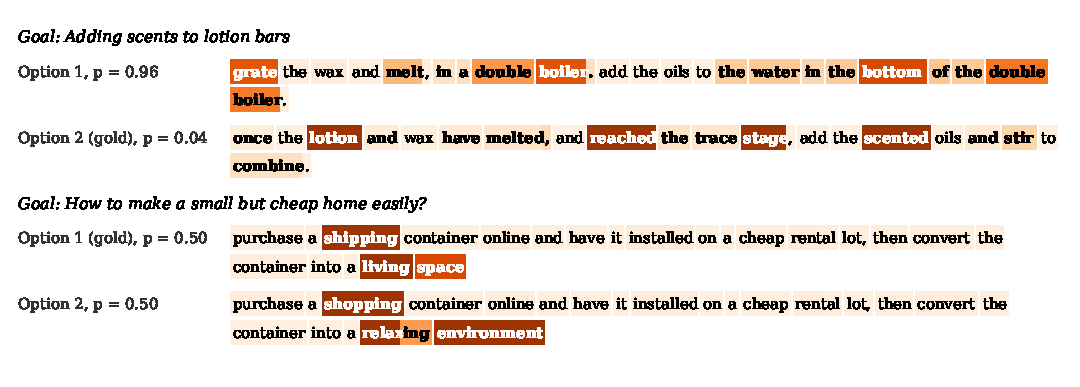
\includegraphics[width=0.98\textwidth]{figures/attention_cases.pdf}
\caption{Pooling attention of the best-validation-seed model over the candidate solutions of two evaluation items (darker shading = higher weight; \textbf{bold} = tokens that differ between the candidates; p = predicted probability). Top: \emph{becoming more mindful}, a correct prediction (p = 0.99 for option 1, the gold answer). Bottom: \emph{adding scents to lotion bars}, an incorrect prediction (p = 0.96 for option 1; option 2 is gold).}
\label{fig:cases}
\end{figure*}

The trained model puts 78.0\% of its pooling attention on differing tokens, which make up 24.8\% of the solution tokens (the notebook plots the full distribution). Because the tag bias starts at 1, two controls separate learned focus from the built-in prior. An untrained model reaches only 38.9\%, whereas the trained model with the bias set to 0 still reaches 62.0\%, and the bias itself barely moved during training (1.0\,$\to$\,1.03). Most of the focus is therefore learned by the pooling scorer, which fits the small effect of initialising the bias at 0. On validation, the normalised pooling entropy is 0.59 (1 = uniform), for correct and wrong predictions alike ($p{=}0.98$). A linear probe for differing versus shared tokens reaches 62.0\% balanced accuracy on the vanilla Transformer's embeddings and only 63.0\% after its encoder, against 100\% in every layer of \dact{}: without tags, the encoder hardly learns where the candidates differ. Wrong predictions place slightly more attention on the differing tokens than correct ones (79.0 vs.\ 77.4\%, Mann--Whitney $p{=}0.03$), so attending to the differing tokens is not sufficient for a correct prediction. Attention weights show where the model puts weight when it aggregates, but they do not by themselves explain why it makes a prediction \cite{jain2019attention,wiegreffe2019attention}.

\subsection{Qualitative Analysis}
Figure~\ref{fig:cases} shows two evaluation items the model predicted confidently, one correctly and one not. In the correct prediction (top), the pooling weight falls on \emph{present}, \emph{meditate} and \emph{moment} in the gold option and on \emph{relax}, \emph{closed} and \emph{focus} in the rival, the content words that set the two activities apart. For \emph{adding scents to lotion bars} (bottom), the wrong option adds the oils ``to the water in the bottom of the double boiler''. The pooling peaks on \emph{bottom}, exactly the part that makes the option wrong, and yet the model prefers this option with p = 0.96: attending to the decisive span did not lead to a correct judgement. In the most uncertain item (p = 0.50; option 1 is gold), shown in the notebook, almost half of the pooling weight sits on a one-letter typo, \emph{shipping} vs.\ \emph{shopping} container, but the two scores are tied. The most confident error (\emph{an exotic trip}, p = 0.98) involves options that share almost no words; because $\ell_k$ sums over n-grams, such spans get extreme lexical scores. Single examples like these illustrate the model's behaviour but do not establish it.

\subsection{Experimental Stability}\label{sec:stability}
The lexical component needed its own learning rate: with the shared rate, its weights barely moved away from zero before early stopping. We also pre-registered a goal-matching block (165\,k parameters) and committed its acceptance rule (validation gain $\geq$ 1.0 point and $>$ 2 pooled seed standard deviations) before training; it lost 0.3 points on validation and was rejected without an evaluation run. Results were sensitive to seeds and sessions. Between the A100 run and the final run, single ablations and the from-scratch baselines moved by up to 1.6 points, the one-seed grid picked a different configuration, and RoBERTa's fine-tuning succeeded in one, two or all three seeds depending on the session. We therefore base our conclusions only on effects larger than this spread.

\subsection{Limitations}\label{sec:limits}
Improvements of about one point are within seed and sampling noise, and each grid candidate was trained with a single seed. The evaluation split was exposed during development (Section~\ref{sec:protocol}), so an untouched estimate of generalisation would need a fresh held-out split. One evaluation item overlaps with the training data, and the difference tags depend on the order of the options (102 evaluation items change tags when the options are swapped; an optional canonical alignment removes this dependence). BPE training in the \texttt{tokenizers} library and the GPU kernels are not deterministic, so re-runs reproduce the results only up to seed-level variation. Finally, the model overfits quickly, reaching 85--92\% training accuracy against about 61\% validation accuracy at the selected epoch, so early stopping does most of the regularisation.

\section{Conclusion}
We built \dact{}, a difference-aware Transformer for PIQA trained from scratch. Making the differences between two near-identical solutions explicit and adding lexical evidence gave the best validation accuracy among the models trained from scratch in two independent runs, but no significant difference from TF-IDF on the evaluation split. The combined design produced the clearest improvement (3.7 / 4.3 points over a vanilla Transformer), while single components had no consistent effect. The model's attention concentrates on the differing words, yet this does not stop it from making confident errors, and pretrained models remain clearly stronger. Our results suggest that, for a model trained from scratch on PIQA, the bottleneck is not finding the relevant difference but judging it, which takes knowledge a training set of 14{,}501 items does not contain. Future work should normalise the lexical score by length, evaluate on a fresh held-out split and transfer the difference-aware mechanisms to pretrained representations.

\section*{Team Contributions}
The work was divided among the three members; each member implemented and tested their own part of the code and wrote the report sections that describe it.

\textbf{Bayron:} original DACT pipeline (data processing, model, training and evaluation code, baselines B0--B4), the original A100 run, the final A100 runs of both versions and their comparison, and integration of the final notebook and report.

\textbf{Ali:} model revision (difference-aware truncation, lexical component and its validation pilot), attention controls and diagnostics, three-seed RoBERTa baseline, the free-T4 runs, and the first draft of the report.

\textbf{Salah:} evidence audit of the original run (training/evaluation overlap, order-dependent alignment, evaluation exposure), robustness and provenance code (validation, determinism, prediction export), and the local replication of the original model.

\clearpage
\bibliography{references}

\end{document}
